\documentclass[paper=a4, fontsize=11pt]{scrartcl} % A4 paper and 11pt font size
\usepackage[utf8]{inputenc}
\usepackage[T1]{fontenc} % Use 8-bit encoding that has 256 glyphs
\usepackage{fourier} % Use the Adobe Utopia font for the document - comment this line to return to the LaTeX default
\usepackage[ngerman,british,UKenglish,USenglish,american]{babel}
\usepackage[utf8]{inputenc}
\usepackage{amsmath,amsfonts,amsthm} % Math packages
\usepackage{hyperref}
\usepackage{fancyhdr}
\usepackage{graphicx}
\usepackage{listings}
\usepackage{todonotes}
\usepackage{titlesec}
\usepackage{xcolor}
\definecolor{grey}{rgb}{0.4, 0.4, 0.4}

%\usepackage{sectsty} % Allows customizing section commands
%\allsectionsfont{\centering \normalfont\scshape} % Make all sections centered, the default font and small caps

\usepackage{fancyhdr} % Custom headers and footers
\pagestyle{fancyplain} % Makes all pages in the document conform to the custom headers and footers
\fancyhead[R]{} % No page header - if you want one, create it in the same way as the footers below
\fancyfoot[L]{} % Empty left footer
\fancyfoot[C]{\thepage} % Page numbering for center footer
\fancyfoot[R]{} % Empty right footer
\renewcommand{\headrulewidth}{0pt} % Remove header underlines
\renewcommand{\footrulewidth}{0pt} % Remove footer underlines
\setlength{\headheight}{13.6pt} % Customize the height of the header

%farbige Hyperlinks
%\definecolor{refcolor}{rgb}{0,.2,.4}
%schwarze Hyperlinks
\definecolor{refcolor}{rgb}{0,0,0}
%Hyperref Color
\hypersetup{pdftex=true, colorlinks=true, breaklinks=true, linkcolor=refcolor, menucolor=refcolor, pagecolor=refcolor, citecolor=refcolor, urlcolor=refcolor}

\numberwithin{equation}{section} % Number equations within sections (i.e. 1.1, 1.2, 2.1, 2.2 instead of 1, 2, 3, 4)
\numberwithin{figure}{section} % Number figures within sections (i.e. 1.1, 1.2, 2.1, 2.2 instead of 1, 2, 3, 4)
\numberwithin{table}{section} % Number tables within sections (i.e. 1.1, 1.2, 2.1, 2.2 instead of 1, 2, 3, 4)

\setlength\parindent{0pt} % Removes all indentation from paragraphs - comment this line for an assignment with lots of text

%----------------------------------------------------------------------------------------
%	TITLE SECTION
%----------------------------------------------------------------------------------------

\newcommand{\horrule}[1]{\rule{\linewidth}{#1}} % Create horizontal rule command with 1 argument of height

\title{	
\normalfont \normalsize 
\textsc{
\includegraphics[width=0.6\textwidth]{pictures/logo} \\ [5pt] Arbeitsgruppe Datenbanken und Informationssysteme \\ [20pt] 
\includegraphics[width=0.15\textwidth]{pictures/DBIS_Logo_rgb_web.png}} \\ [10pt] % Your university, school and/or department name(s)
\horrule{0.5pt} \\[0.4cm] % Thin top horizontal rule
\huge Spatial Databases: Project Documentation \\ % The assignment title
\normalsize \textsc{Setup-Guide and Documentation for Spatial-Weather-Project} \\ [0.4cm]
\horrule{2pt} \\[0.5cm] % Thick bottom horizontal rule
}
\newcommand*{\justifyheading}{\raggedright}
\titleformat{\subsection}{\large\justifyheading}{\thesubsection}{1em}{}

\author{Johannes Dillmann (matr-nr) \\ Christian Wirth (4498611) \\ Jens Fischer (matr-nr)}

\date{\normalsize\today} % Today's date or a custom date
\begin{document}

\begin{titlepage}
\pagenumbering{Roman}
\maketitle
\thispagestyle{empty}
\end{titlepage}

\newpage
\setcounter{page}{1}
\addcontentsline{toc}{section}{\protect\numberline{}{Table of Contents}}
\tableofcontents
%\thispagestyle{empty}

\newpage
\listoffigures
\addcontentsline{toc}{section}{\protect\numberline{}{Table of Figures}}

\newpage
\pagenumbering{arabic}
\pagestyle{fancy}
\setcounter{page}{1}

\section{Introduction}
	\subsection{Topic}
	The topic of this project is to combine OSM-data provided by Open Street Maps and weather-Data on a spatial database server running PostGIS.
	\subsection{Motivation}
	The motivation of this project can be seen from a educational as well as from a technical point of view.\\
	The educational purpose of this project is to encourage the students to acquire domain-knowledge concerning the problem that needs to solved with a system that is requested to be set up. In this particular case the domain is weather-data. By working hands-on with real data the students expand their range of skills in order to be able to work with problems that exceed the boundary of purely computational and mathematical problems. This focuses on an important trade every programmer will need once he lives university and has to deal with real world problems.\\
	Once these domain-related problems are understood the students face the technological challenges in order to find a solution to the given problem which will be explained in the following subsection.
	\subsection{Goal}
	The Goal is to find suitable sources for weather-forecast and historical weather-data as well as storing it on a PostGIS-server. In the end the system shall be able to overlay the OSM- and the collected weather-data. In order to achieve this Goal several technical Problems have to be solved, like designing a Data-Model, a suitable System-Architecture as well as setting up and configuring the whole System.
	
\newpage
\section{Data Sources}\label{sec:datasources}
	- kurze Beschreibung der drei Datenquellen
	- vielleicht die (konzeptuelle) Beschreibung der Download Prozesse auch hier?
	
\section{Data Model}
\begin{figure}[htbp]
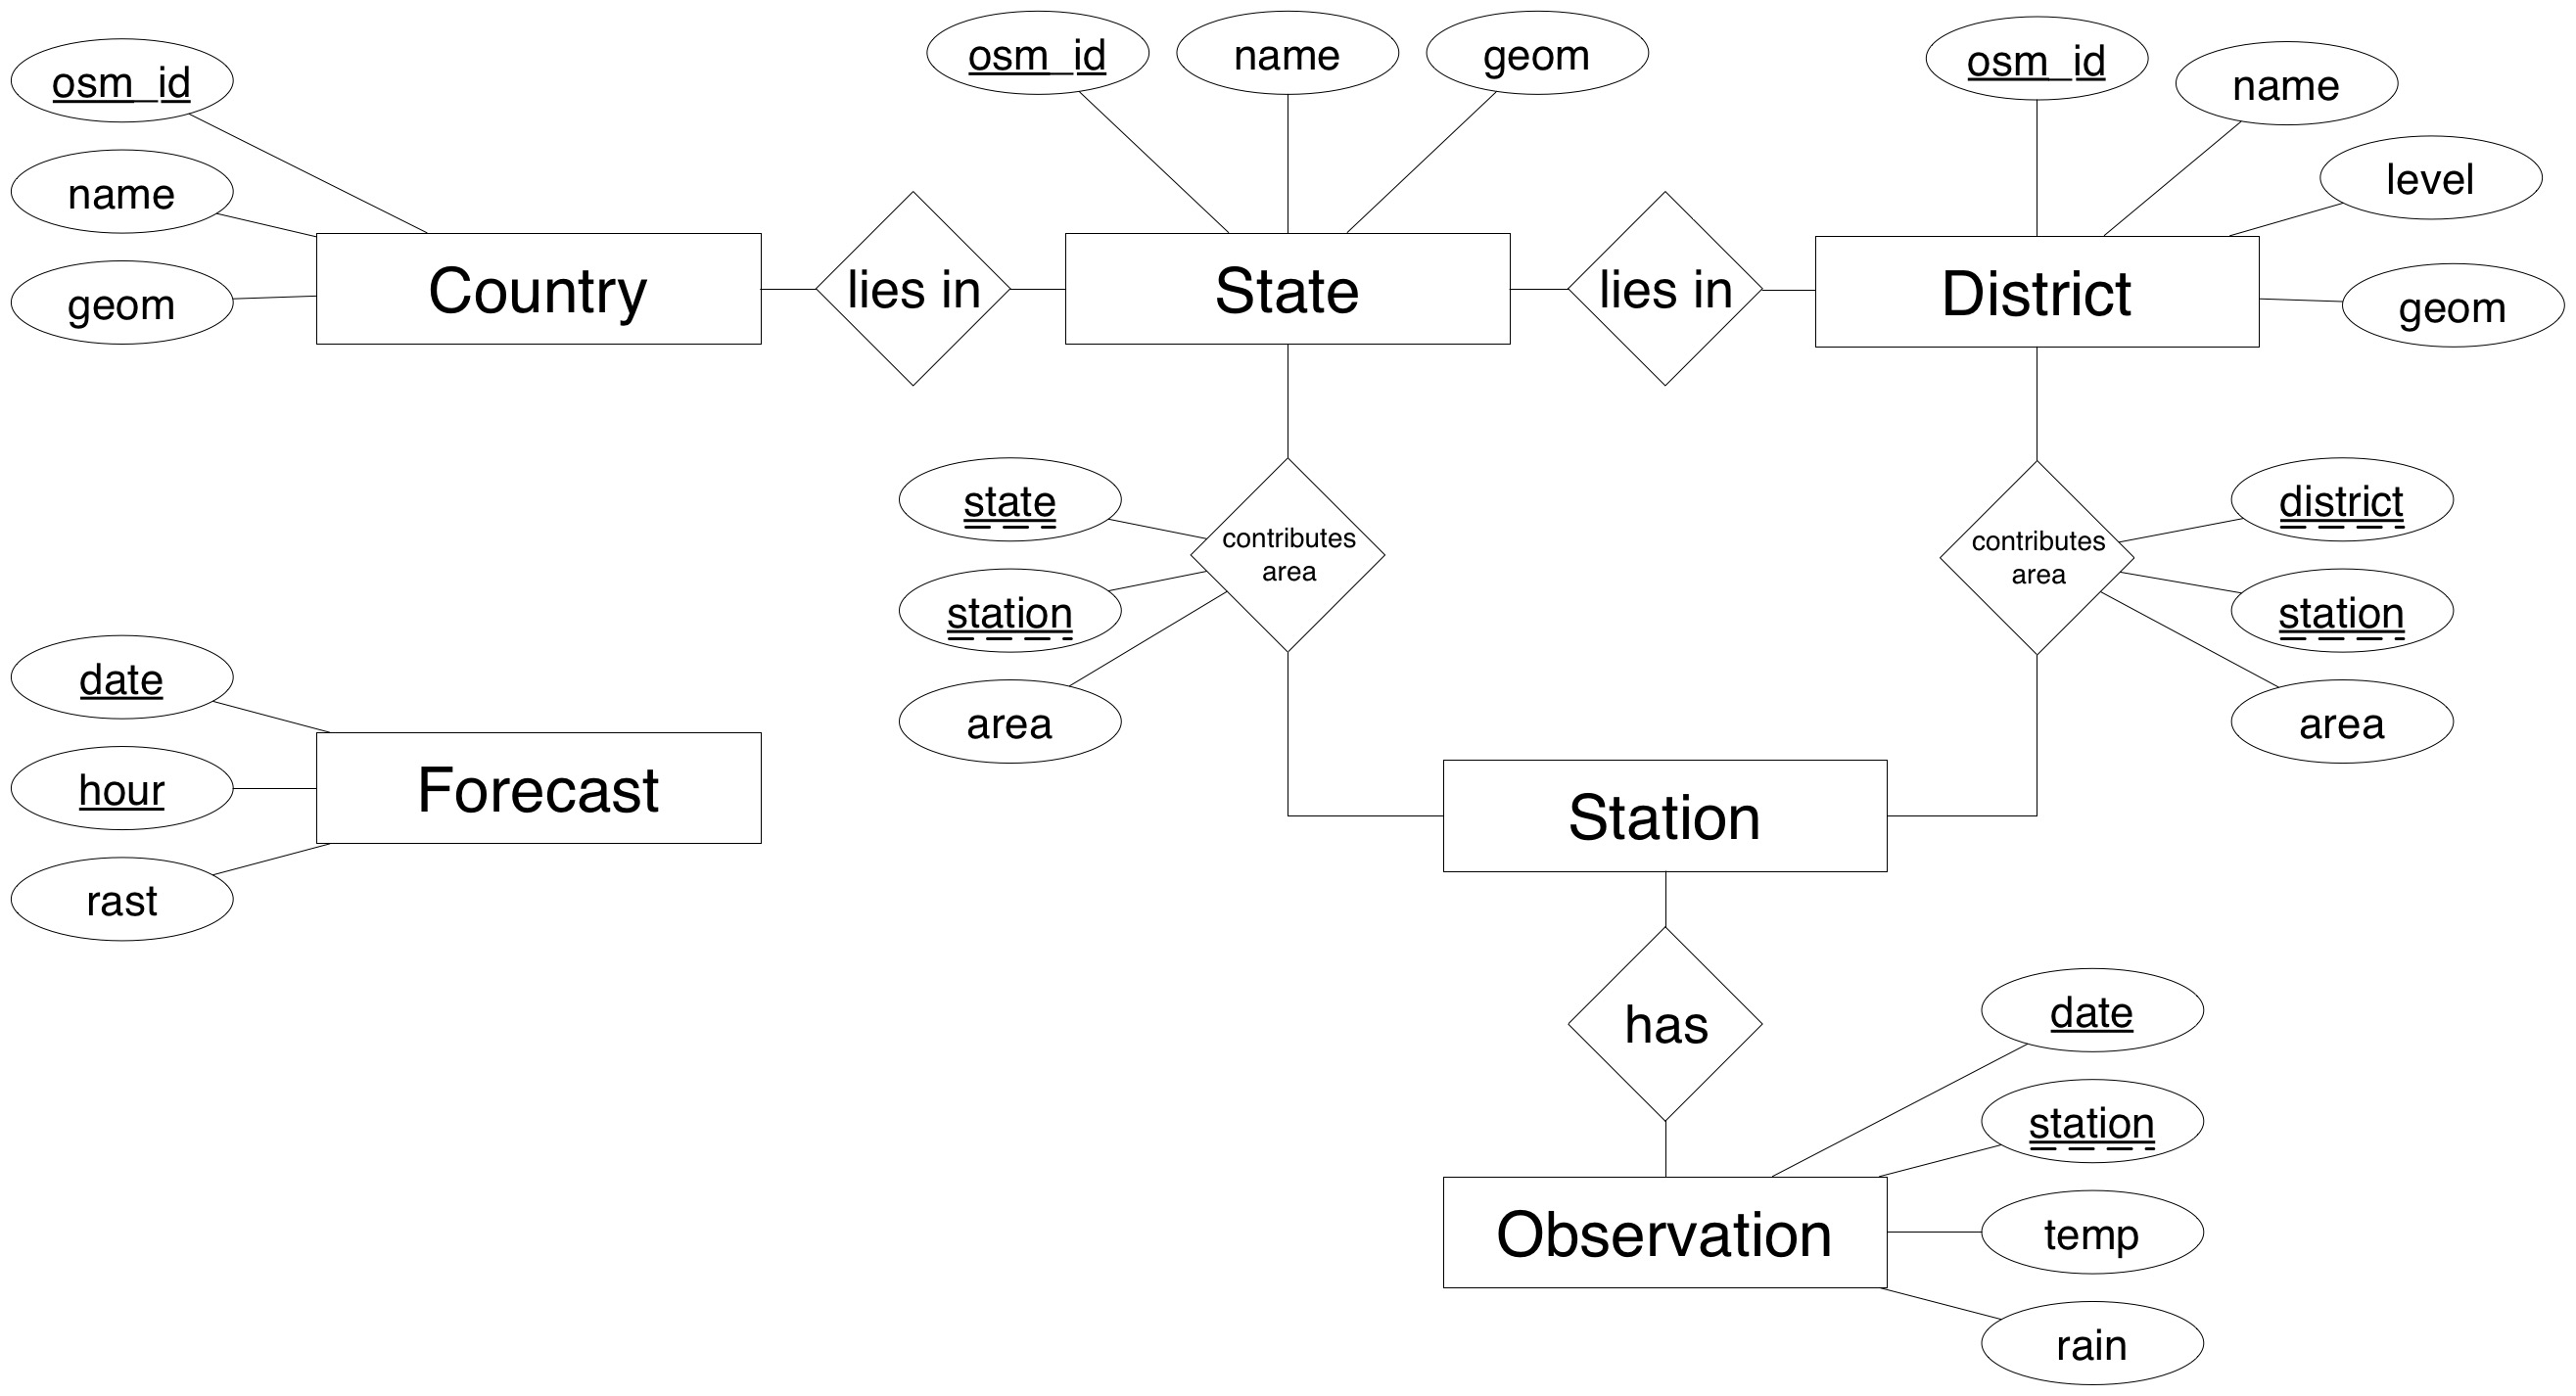
\includegraphics[width=1\textwidth]{pictures/ER}
\caption{ER-Diagram}
\end{figure}

\newpage
\section{Architecture}
The Architecture as shown in fig. \ref{fig:architecture} consist of 4 major parts:\\
The data-sources and their corresponding downloaders and importers, the PostGIS-Server, running in a virtual machine, the backend and a webapp. In the following four subsections \ref{subsec:dsai} to \ref{subsec:webapp} I'll explain how those components are working together and what parts they are made of as well as which technologies have been used to implement them.
\begin{figure}[htbp]
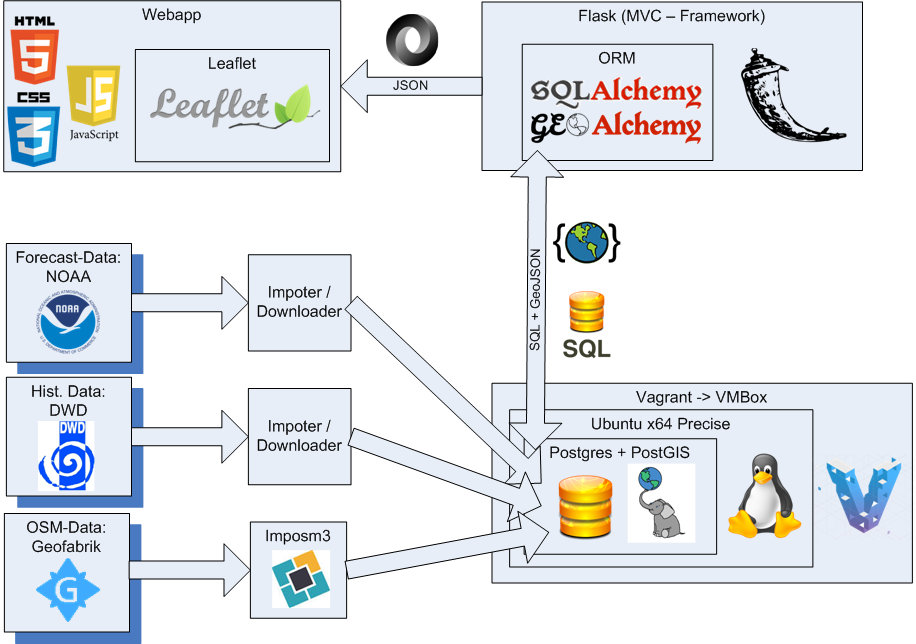
\includegraphics[width=1\textwidth]{pictures/Architektur.png}
\caption{Architecture}
\label{fig:architecture}
\end{figure}
\todo[inline]{Schreibfehler korrigieren}

\subsection{Data Sources and Importer}\label{subsec:dsai}
The three data-sources used in this project are \todo[inline]{add 3 sources} and have been discussed in section \ref{sec:datasources} very detailed. The importers write the collected data directly to the spatial database server so they can be used to answer the queries by the backend. For further information on this part please refer to section \ref{sec:datasources} and the setup-guide at subsections \ref{import-osm-data} to \ref{download-and-import-noaa-gfs-data-forecasts}
\subsection{Server}
The server is provided as Vagrant virtual machine. Vagrant is a tool to automate the setup of virtual machines. In this case vagrant initializes a Ubuntu x64 instance and installs postgres and PostGis along with other required packages and configures most of the things needed for the server to be ready to be used.
\subsection{Backend}
The backend runs Flask, a model-view-controller-based framework. This framework contains methods to invoke data-collection and data-import as well as an ORM based on SQL-Alchemy and GEO-Alchemy to send queries to the database to retrieve data requested by the user via the Frontend. The queries are written in python, the ORM translates those queries to SQL and the the response from the database is converted to GeoJSON, which is then forwarded to the Frontend.
\subsection{Webapp (Frontend)}\label{subsec:webapp}
The Frontend in implemented as a webapp written in HTML5, CSS3 and Javascript and provides a User Interface which is described in detail in section \ref{usage}. To display the weather- and OSM-data the library Leaflet is used. The Frontend receives the requested data from the backend in JSON.

\section{Optimizations}
	- Indices
	- Contrib Tables
	- Topology Simplification
\section{Usage}\label{usage}

As mentioned in the architecture section, the weather map is displayed
with HTML5 and controlled with JavaScript. It has been developed as a
control for the Leaflet library and tested on Google Chrome and
Chromium. Other browsers are not officially supported.

By default Leaflet is using a zoom and a layer selection control.
Instead of rendering the base tiles ourselves, we are using the freely
available
\todo[inline]{Sources}
\href{http://wiki.openstreetmap.org/wiki/Tile_usage_policy}{OSM Tile
Server} and tiles generated for free by
\href{https://www.mapbox.com/}{Mapbox}. The desired basetile layer can
be selected as seen in fig. \ref{fig:layer-selection}

\begin{figure}[htbp]
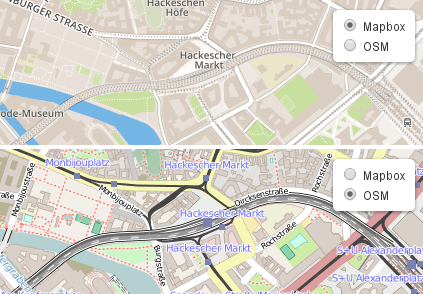
\includegraphics[width=1\textwidth]{pictures/screenshot-baselayer.png}
\caption{Layer selection}
\label{fig:layer-selection}
\end{figure}

\newpage
The map can also be panned and zoomed by using a pointing device
(e.g.~mouse).

The displayed weather data can be set by an additional control as seen
in fig. \ref{fig:weather-control}

\begin{figure}[htbp]
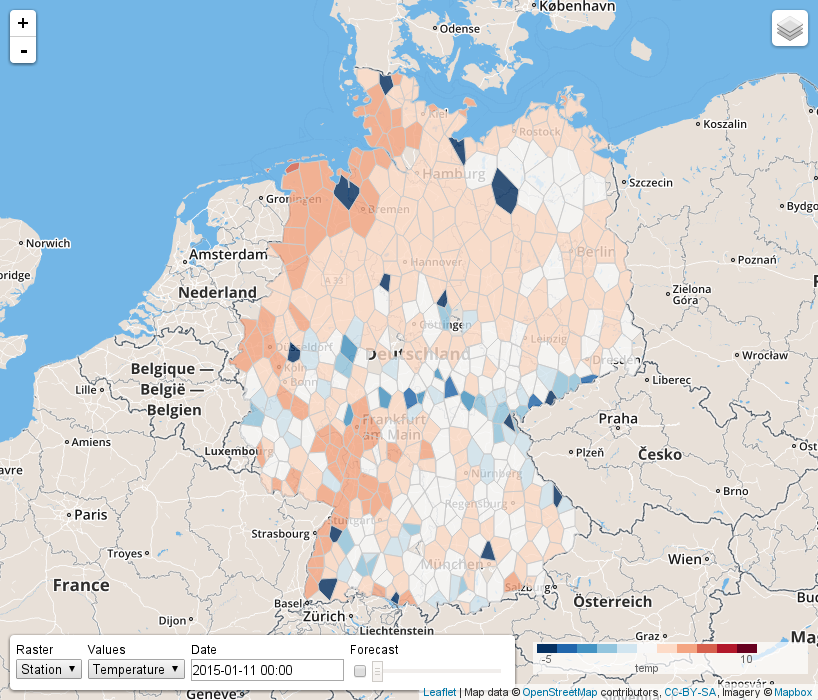
\includegraphics[width=1\textwidth]{pictures/screenshot-control.png}
\caption{Weather control}
\label{fig:weather-control}
\end{figure}

\newpage
It allows to choose either temperatures or reciprocal rainfall for a
certain day. The day can be selected with an interactive date-time picker
as seen in fig. \ref{fig:date-time-picker}

\begin{figure}[htbp]
\centering
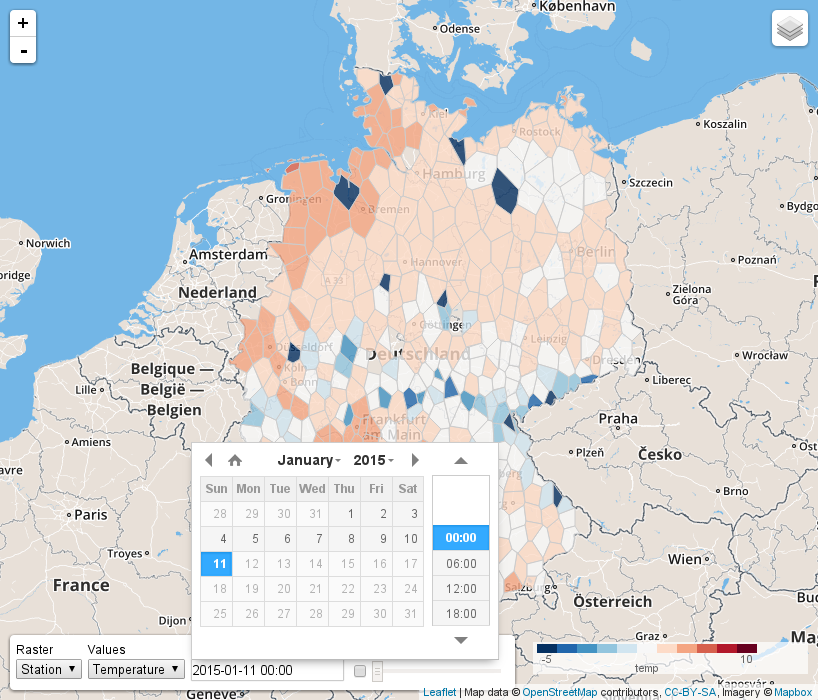
\includegraphics[width=1\textwidth]{pictures/screenshot-control-datetime.png}
\caption{Date-time picker}
\label{fig:date-time-picker}
\end{figure}

The selected date and time is also used to pick the computed GFS used to
display forecasts. If the forecast box is checked, the forecasts slider
is activated and allows to select point of forecast in hours, starting
from the chosen date and time.

\newpage
As mentioned before, the data can be displayed for different rasters: a
voronoi tessellation based on official weather stations, german states or
districts as shown in fig. \ref{fig:raster-comparison}. The desired raster can be selected with the control. Once the
selection did change, the weather control is loading the matching data
from the backend via a JSON interface and displays the raster on the
map.

\begin{figure}[htbp]
\centering
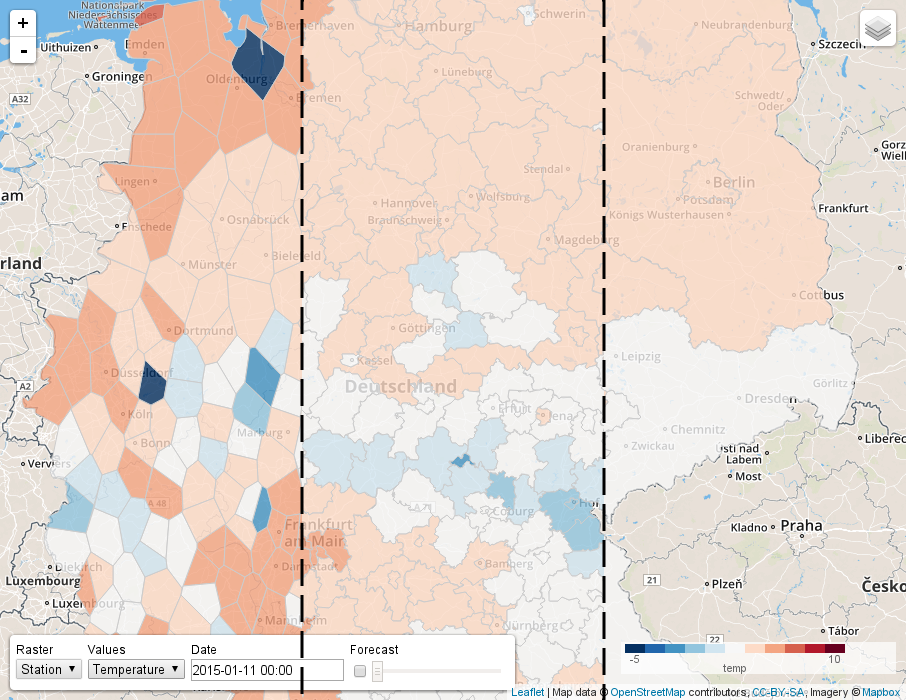
\includegraphics[width=1\textwidth]{pictures/screenshot-raster.png}
\caption{Raster comparison}
\label{fig:raster-comparison}
\end{figure}

The cells are colored according to selected data and a legend is shown
on the lower right for reference (see fig. \ref{fig:temperature-legend} and \ref{fig:rainfall-legend})

\begin{figure}[htbp]
\centering
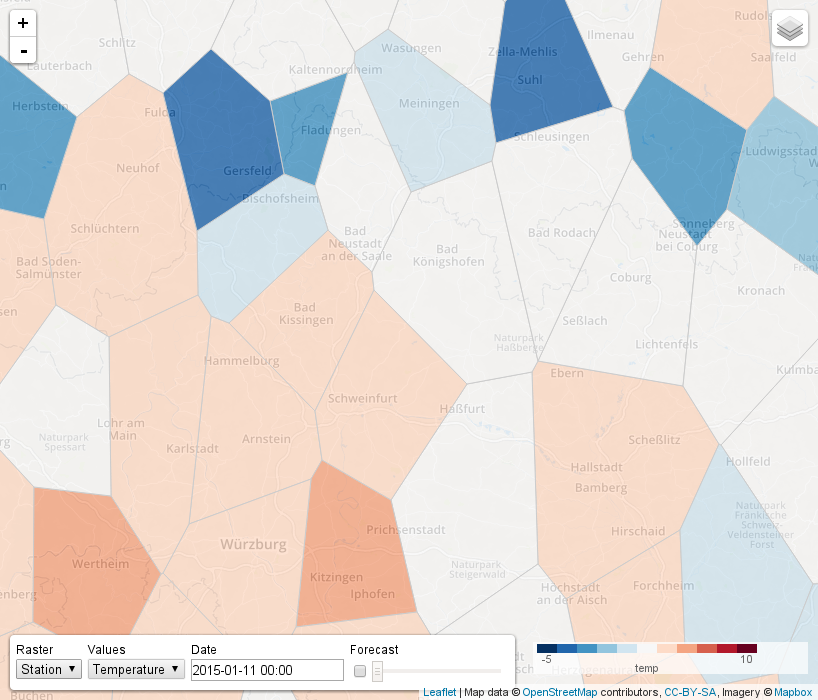
\includegraphics[width=0.5\textwidth]{pictures/screenshot-legend-temp.png}
\caption{Temperature legend}
\label{fig:temperature-legend}
\end{figure}

\begin{figure}[htbp]
\centering
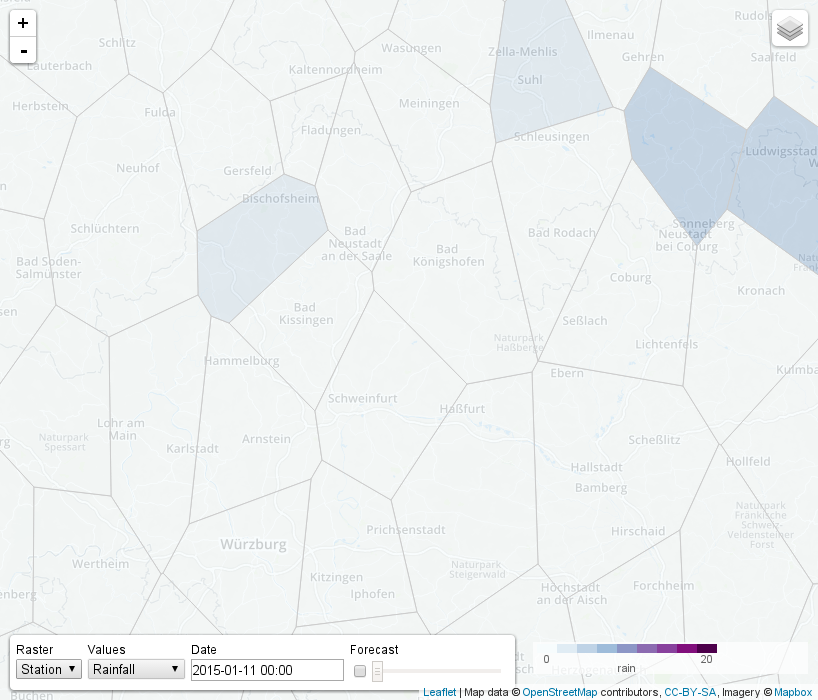
\includegraphics[width=0.5\textwidth]{pictures/screenshot-legend-rain.png}
\caption{Rainfall legend}
\label{fig:rainfall-legend}
\end{figure}

\newpage
Each cell is clickable and highlights it's border or, in case of the
voronoi tessellation, the position of the weather station. Furthermore a
pop-up as in fig. \ref{fig:popup} is shown, which provides additional data associated to the
selected cell by calling the backends JSON interface.

\begin{figure}[htbp]
\centering
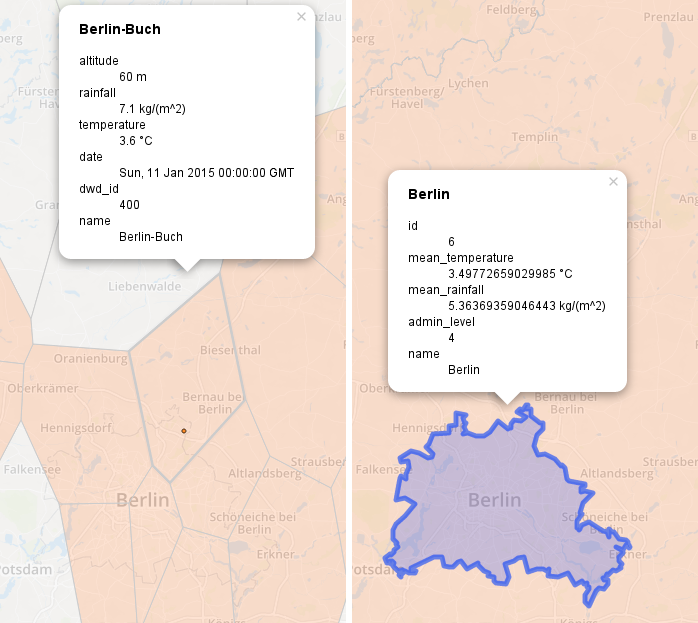
\includegraphics[width=1\textwidth]{pictures/screenshot-popup.png}
\caption{Pop-up}
\label{fig:popup}
\end{figure}

Currently this is just the alphanumerical attributes, but could be used
to show automatically generated temperature timelines or recent webcam
photos or \ldots{}\todo [inline]{noch mehr ausblick kram\ldots}

\section{Conclusion}
	- lessons learned

\section{Setup Guide}
\subsection{Prerequisites}

This Setup-Guide has been writen for and tested with Ubuntu 14.10 'Utopic Unicorn'.\\
The Following Packages or Programs need to be installed before you proceed with this set-up-guide: Git, Vagrant, Python 3, PostGIS

\begin{lstlisting}
sudo apt-get install gdal-bin postgis git vagrant python
\end{lstlisting}
\todo[inline]{check packages}

It is strongly advised to install scipy, numpy and shapely (globaly) as
binary packages and not through virtualenv, because of their large
number of non-python dependencies. E.g. on Debian/Ubuntu systems use
\begin{lstlisting}
sudo apt-get install python3-numpy python3-scipy python3-shapely
\end{lstlisting}
to install. Make sure access to the global packages is activated in the
virtual environment\\(e.g.~through \texttt{toggleglobalsitepackages} in
\texttt{virtualenvwrapper}).

When compiling entirely from source, You also might need to install the
following libraries: (for shapely): libgeos-dev; (for scipy):
libblas-dev, liblapack-dev, gfortran.

\subsection{Step-by-step Setup}
Now switch to directory that should later contain your project-source-code

Clone Repository by typing into console:
\begin{lstlisting}
git clone https://<<your_username>>@bitbucket.org/kleingeist/spatial-weather.git
\end{lstlisting}

Change directory to spatial-weather
\begin{lstlisting}
cd spatial-weather
\end{lstlisting}

Install and configure the virtual machine by entering in console:
\begin{lstlisting}
vagrant up
\end{lstlisting}

You can open a new console and proceed with the following steps on your local machine:\\
Install miniconda from the website:\\
http://conda.pydata.org/miniconda.html

--conda install --file requirements.conda

This command has to be executed every time the server has been started in order to activate the Python virtual environment.
\begin{lstlisting}
source ~/miniconda3/bin/activate spatial-weather
\end{lstlisting}

install database-driver for python3:
\begin{lstlisting}
sudo apt-get install python3-psycopg2 libpq-dev python3-dev
\end{lstlisting}

install additional requirements for python:\\
(take a look at requirements.txt for further details.)
\todo[inline]{TDOD}
\begin{lstlisting}
pip install -r requirements.txt
\end{lstlisting}

These steps will only work once the Virtual Machine has been successfully provisioned.\\
Create database and Postgis extesions:
\begin{lstlisting}[breaklines=true]
vagrant ssh -c "sudo -u postgres psql -c \"CREATE DATABASE spatial OWNER myapp LC_COLLATE 'en_US.UTF-8' LC_CTYPE 'en_US.UTF-8';\"" 
vagrant ssh -c "sudo -u postgres psql -d spatial -c \"CREATE EXTENSION postgis; CREATE EXTENSION postgis_topology;\"" 
vagrant ssh -c "sudo -u postgres psql -d spatial -c \"GRANT ALL ON DATABASE spatial TO myapp; ALTER DATABASE spatial OWNER TO myapp; ALTER TABLE topology OWNER to myapp; ALTER TABLE layer OWNER to myapp; ALTER SCHEMA topology OWNER TO myapp;\""
\end{lstlisting}

\subsection{Import OSM Data}\label{import-osm-data}

Imports the OSM data for Germany. The following tables are created:
Country, State, District and Cities. The data is imported from
\texttt{germany-latest.osm.pbf}, obtained from\\
\href{http://download.geofabrik.de/europe/germany-latest.osm.pbf}{http://download.geofabrik.de/europe/germany-latest.osm.pbf}.
\todo[inline]{Quelle: (last access: 05.02.15)} The pbf file needs to be
placed in \texttt{data/} located in your Project-Folder.

The importer used is \texttt{imposm3}, which is included in the vagrant
setup (and will be executed within the VM). The import\\uses a custom
mapping, which is provided in \texttt{importer/mapping.json}. The import
is conducted in two steps: First, the\\data is imported to the tables
Osm\_Admin and Osm\_Places. Second the Country, State, District and
Cities tables are created\\from these tables.

\subsubsection*{Usage}\label{usage}

Prerequisite: No contrib tables, delete if existing:\\ python manage.py
drop\_tables -t contrib

To import all the OSM data use the manage script. To invoke the whole
pipeline use the following command (will take several hours):

\texttt{python\ manage.py\ import\_osm\ -\/-imposm\ -\/-simplify\ -\/-load\ -\/-drop\_tables}

\begin{itemize}
\itemsep1pt\parskip0pt\parsep0pt
\item
  \texttt{-\/-imposm} the first import step (see above)
\item
  \texttt{-\/-simplify} simplify all map data (borders)
\item
  \texttt{-\/-load} the second import step (see above)
\item
  \texttt{-\/-drop-tables} deletes the Osm\_Admin and Osm\_Places tables
  after a successful import
\end{itemize}

All the above steps can be invoked separately.

\subsubsection*{Mac OS X}\label{mac-os-x}

\begin{lstlisting}[breaklines=true]
python manage.py import_osm --drop_tables --imposm --load
DYLD_LIBRARY_PATH=/Applications/Postgres.app/Contents/Versions/9.3/lib python manage.py import_osm --drop_tables --load
\end{lstlisting}

\subsection{Import DWD Data (Historical)}\label{import-dwd-data}

Imports weather observation data from the DWD (Deutscher Wetterdienst).
The importer is a adopted version
from \href{https://github.com/cholin/fuberlin_spatial_db_project}{cholin}.
\todo[inline]{Quelle}
Per default, it downloads all the {[}recent daily
observations{]}\\(\url{ftp://ftp.dwd.de/pub/CDC/observations_germany/climate/daily/kl}).

Details on the importer from
\href{https://github.com/cholin/fuberlin_spatial_db_project/blob/master/scripts/dwd/README.md}{cholin}:
\todo[inline]{Quelle}

\begin{quote}
The importer downloads the station summary file to get a list of all
weather stations. After that it downloads for each\\station the
corresponding zip file (with measurement data), extracts it in-memory
and parses it. To get information about\\which weather station is the
nearest for a given point, it also calculates a region polygon for each
station. This is done\\by computing the voronoi diagram for all
stations. The resulting regions may be outside of the country germany.
To avoid\\this there is a polygon of the border of germany (data is from
naturalearthdata.com - country extraction and exportation\\as geojson
with qgis). For each region we calculate the intersection with this
polygon and use the result as final region\\(Multi)Polygon.
\end{quote}

\subsubsection*{Usage}\label{usage-1}

Use the importer with the \texttt{manage.py} script:

To download all data and import all observation data:

\texttt{python\ manage.py\ import\_dwd}

Create an intermediate result in \texttt{data/weather.json}:

\texttt{python\ manage.py\ import\_dwd\ -\/-to\_json}

Import the intermediate result from \texttt{data/weather.json}:

\texttt{python\ manage.py\ import\_dwd\ -\/-from\_json}

\subsubsection*{Mac OS X}\label{mac-os-x-1}

\begin{lstlisting}[breaklines=true]
python manage.py import_dwd --to_json
DYLD_LIBRARY_PATH=/Applications/Postgres.app/Contents/Versions/9.3/lib ython manage.py import_dwd --from_json
\end{lstlisting}

\subsection{Download and Import NOAA GFS Data
(Forecasts)}\label{download-and-import-noaa-gfs-data-forecasts}

Importing the Forecast Data is done in two steps. First you have to
download the GRIB files from the NOAA FTP servers. Then you have to
import them as Postgis Raster.

\subsubsection*{Download}\label{download}

For downloading the GFS data a date range and a target directory has to
be specified. The format for the start and enddate is
\texttt{YYYYMMDDHH} or \texttt{latest} for the most recently available
GFS calculation.\\Optionally the forecast hours can be specified as a
range (Defaults to download from 0 to 129 in 3 hour steps).

\begin{verbatim}
usage: run_gfs.py download [-h] [--hours_start HOURS_START]
                           [--hours_stop HOURS_STOP] [--hours_step HOURS_STEP]
                           [startdate] [enddate] datadir
\end{verbatim}

For example, assuming data should be stored to \texttt{data/forecasts}:

\texttt{./run\_gfs.py\ download\ 2014121112\ 2015011306\ data/forecasts}

\subsubsection*{Import}\label{import}

To import the downloaded data, the download directory and a data range
has to be specified:

\begin{verbatim}
usage: run_gfs.py import [-h] datadir [startdate] [enddate]
\end{verbatim}

For example, assuming the data is stored in \texttt{data/forecasts}:

\texttt{./run\_gfs.py\ import\ data/forecasts\ 2014121112\ 2015011306}

\subsubsection*{Build Contrib Tables}\label{build-contrib-tables}

To speed up some queries, the area contribution of the region (voronoi
cell) of weather stations to states and districts is precomputed and
materialized. \\
Run \texttt{python\ manage.py\ calculate\_contrib\_area}
to create and fill the ContribState and ContribDistrict tables.

\subsubsection*{Troubleshooting (Mac OS X)}\label{troubleshooting}

\subsubsection*{UnicodeEncodeError}\label{unicodeencodeerror}

Python inherits the standard locale from the current shell environment.
If this is not set to utf8 it tries to convert to ASCII, which
produces.\\
\texttt{UnicodeEncodeError:\ \textquotesingle{}ascii\textquotesingle{}\ codec\ can\textquotesingle{}t\ encode\ character}\\Test
with \texttt{\$\ locale}, this should show utf-8. If not, fix with
\begin{verbatim}
export LANG=en_US.UTF-8
export LC_ALL=en_US.UTF-8
\end{verbatim}

\subsubsection*{libssl / libcrypto Error from
psycopq}\label{libssl-libcrypto-error-from-psycopq}

The \texttt{libssl} version Mac OS X uses might be too old for
\texttt{psycopg}, resulting in an error like the following:

\begin{lstlisting}[breaklines=true]
...
ImportError: dlopen(...lib/python3.4/site-packages/psycopg2/_psycopg.so, 2): Library not loaded: libssl.1.0.0.dylib
  Referenced from: ...lib/python3.4/site-packages/psycopg2/_psycopg.so
  Reason: image not found
\end{lstlisting}

This can be solved by changing the dynamic shared library install names
in the \texttt{psycopq} binary. First, find out the version
\texttt{psycopq} is using:

\begin{lstlisting}[breaklines=true]
otool -L /Users/jvf/miniconda3/envs/env-sw/lib/python3.4/site-packages/psycopg2/_psycopg.so
$ /Users/jvf/miniconda3/envs/env-sw/lib/python3.4/site-packages/psycopg2/_psycopg.so:
    /usr/local/lib/libpq.5.dylib (compatibility version 5.0.0, current version 5.6.0)
    libssl.1.0.0.dylib (compatibility version 1.0.0, current version 1.0.0)
    libcrypto.1.0.0.dylib (compatibility version 1.0.0, current version 1.0.0)
    /usr/lib/libSystem.B.dylib (compatibility version 1.0.0, current version 1213.0.0)
    /usr/lib/libgcc_s.1.dylib (compatibility version 1.0.0, current version 283.0.0)
\end{lstlisting}

Now, change the the shared libraries for \texttt{libssl} and
\texttt{libcrypto} (using the libraries provided by
\href{http://postgresapp.com}{Postgres.app}):

\begin{lstlisting}[breaklines=true]
install_name_tool -change libssl.1.0.0.dylib /Applications/Postgres.app/Contents/Versions/9.3/lib/libssl.1.0.0.dylib /Users/jvf/miniconda3/envs/env-sw/lib/python3.4/site-packages/psycopg2/_psycopg.so
install_name_tool -change libcrypto.1.0.0.dylib /Applications/Postgres.app/Contents/Versions/9.3/lib/libcrypto.1.0.0.dylib /Users/jvf/miniconda3/envs/env-sw/lib/python3.4/site-packages/psycopg2/_psycopg.so
\end{lstlisting}

\texttt{psycopq} now uses the correct libraries:

\begin{lstlisting}[breaklines=true]
otool -L /Users/jvf/miniconda3/envs/env-sw/lib/python3.4/site-packages/psycopg2/_psycopg.so                                                                                                                                                   
$ /Users/jvf/miniconda3/envs/env-sw/lib/python3.4/site-packages/psycopg2/_psycopg.so:
    /usr/local/lib/libpq.5.dylib (compatibility version 5.0.0, current version 5.6.0)
    /Applications/Postgres.app/Contents/Versions/9.3/lib/libssl.1.0.0.dylib (compatibility version 1.0.0, current version 1.0.0)
    /Applications/Postgres.app/Contents/Versions/9.3/lib/libcrypto.1.0.0.dylib (compatibility version 1.0.0, current version 1.0.0)
    /usr/lib/libSystem.B.dylib (compatibility version 1.0.0, current version 1213.0.0)
    /usr/lib/libgcc_s.1.dylib (compatibility version 1.0.0, current version 283.0.0)
\end{lstlisting}

It is strongly recommended to do all this in an virtual environment to
not mess up your system!

Source: More Information:
\href{http://superuser.com/a/721564}{superuser.com}

Another possibilty is to prefix commands with
\texttt{DYLD\_LIBRARY\_PATH} and \texttt{DYLD\_FRAMEWORK\_PATH}, but
this works less reliable and potentially messes up the linking of other
libraries. Example:

\begin{lstlisting}[breaklines=true]
DYLD_LIBRARY_PATH=$(HOME)/lib:/usr/local/lib:/lib:/usr/lib:/Applications/Postgres.app/Contents/Versions/9.3/lib,DYLD_FRAMEWORK_PATH=/Library/Frameworks:/Network/Library/Frameworks:/System/Library/Frameworks python manage.py import_dwd
\end{lstlisting}

providing an alternative path for a newer version of \texttt{libssl} to
the dynamic linker (in this example the libs from
\href{http://postgresapp.com}{Postgres.app} are used, but can link
against a \texttt{homebrew} installed version as well):

\begin{lstlisting}[breaklines=true]
export DYLD_LIBRARY_PATH=$(HOME)/lib:/usr/local/lib:/lib:/usr/lib:/Applications/Postgres.app/Contents/Versions/9.3/lib
export DYLD_FRAMEWORK_PATH=/Library/Frameworks:/Network/Library/Frameworks:/System/Library/Frameworks
\end{lstlisting}

Source:
\href{http://stackoverflow.com/questions/11365619/psycopg2-installation-error-library-not-loaded-libssl-dylib}{stackoverflow.com}

\todo[inline]{TODO}

\subsection{Start Webapp-Server}
Remember to set the virtual environment first if you restarted the Virtual Machine.
\begin{lstlisting}
source ~/miniconda3/bin/activate spatial-weather
\end{lstlisting}
Then you can run the Webserver:
\begin{lstlisting}
python manage.py runserver
\end{lstlisting}

\section{Appendix}
\todo [inline] {Literature (if any)}
\subsection{Link to Repository}

\end{document}
